Este capitulo tiene como objeto introducir los conocimiento sobre sistemas de posicionamiento Global (GPS) y los aspectos técnicos relacionados con la señales y su recepción en dispositivos de posicionamiento (receptores).

\section{Sistema global de posicionamiento satelital - GNSS}

El sistema de posicionamiento global (GPS), es el primer sistema global de navegación satelital GNSS. GPS consta de una constelación de 24 satélites sobre la orbital media de la tierra que trasmite continuamente señales de radio frecuencia hacia la tierra, permitiendo así que los dispositivos de posicionamiento puedan determinar su posición sobre la superficie terrestre.\\

La idea detrás de los sistemas de posicionamiento tales como GPS, puede resumirse en que:

\textit{Si la distancia desde tres satélites en el espacio a un punto en común sobre la superficie de la tierra(un receptor GPS) es conocida, junto con la posición de los satélites al momento de la transmisión, la posición del receptor puede ser determinada gracias a la aplicación de conceptos trigonométricos, álgebra y un sistema de coordenadas apropiado.\cite{Thompson_1998}.}

Sin embargo, la problemática es ¿Como conseguir las distancias a cada satélite de forma precisa, para poder aumentar la precisión al momento de determinar la posición del receptor sobre la superficie de la tierra.?\\

Para ello es necesario profundizar mas los conceptos y conocimientos acerca del funcionamiento de GPS.\\

\subsection{El funcionamiento}

GPS funciona gracias a la transmisión continua de señales de radiofrecuencia a través de la ionosfera y la troposfera. Las señales transmitidas están conformadas por dos señales de portadora, dos códigos y un mensaje de navegación (detalles acerca del satélite). Estas señales son adquiridas gracias una antena especialmente diseñada para captar la señales en el rango de frecuencias específicos en que transmiten los satélites GPS (1227.60 y 1575.42 MHz). Posterior a la adquisición y decodificación de la señal viene una etapa de cálculos en la que un componente de software realiza cálculos para descifrar que mensaje de navegación corresponde a determinado satélite, gracias a los códigos recibidos de manera simultanea.


\subsection{Representación numérica de las señales}

En teoría, una vez las señales han sido decodificadas y clasificadas, con el conocimiento de las distancias de tres satélites hasta el punto donde se ubica el receptor, es posible mediante la solución a un sistema de ecuaciones que tiene como incógnitas las coordenadas X, Y, Z donde se encuentra el receptor. Sin embargo, un cuarto satélite es necesario para una cuarta variable (tiempo), la cual hace referecia al momento exacto en el que el receptor recibir las señales que le permiten posicionarse.



\subsection{Triangulación y trilateración}

Triangulación es el método o forma más común para la  determinación de una posición sobre la superficie terrestre basada en puntos de referencias o “faros”. Para ello, los ángulos entre el receptor y los puntos de referencia deben ser conocidos para que receptor puede determinar su posición; en este escenario, la precisión con la que el receptor determina su posición, depende de la precisión con la que puede medir los ángulos con respecto a cada punto de referencia.\\
 
La Trilateración, es un método apoyado en el conocimiento de las posiciones de los puntos de referencia. En este caso, la precisión con la que el receptor puede determinar su posición depende estrictamente de la exactitud con la que puede medir la distancia hasta el punto de referencia. En este concepto se apoya el funcionamiento de GPS.
\\
Definición de la distancia entre receptor los puntos de referencia (satélites),  se vale de medir la duración del viaje de una señal proveniente del espacio hasta el receptor a través de las atmósfera. Los conceptos de entradas del cálculo de la distancia de viaje de la señal son conceptos que van a ser profundizados en la teoría del funcionamiento de los sistemas de posicionamiento satelital en (libro tal y tal).\\

Es importante aclarar que el nivel de precisión con que los receptores GPS pueden determinar su posición sobre la tierra depende ya no solo de la precisión con que mide los tiempos de viaje de la señal, ya que fenómenos físicos involucrados en el viaje de la señal, errores en la sincronización de reloj en los satélites y el receptor y demás, afectan la exactitud con que se determina el tiempo de viaje al momento de la recepción induciendo errores en la determinación de la distancia y por ende error en el cálculo de posicionamiento de recetor a partir de estas mediciones.\\

El perfeccionamiento de modelos matemáticos, técnicas de posicionamiento y avances tecnológicos en los receptores GPS, tienen como único objeto la mitigación de los errores inducidos en la determinación del tiempo de viaje en la señal, para así mejorar la precisión en el posicionamiento.\\

\section{Modelos observacionales y técnicas de posicionamiento}

La variedad de observables de medición arrojado por los dispositivos de posicionamiento son el resultado de los procedimientos internos del receptor para la estimación de los tiempos de viaje de la señal, luego de las etapas de adquisición y de-modulación, que pueden estar expresados en estándares como \textbf{NMEA\footnote{NMEA: National Marine Electronics Association,  http://www.gpsinformation.org/dale/nmea.htm}} y \textbf{RINEX\footnote{RINEX: Receiver INdependent EXchange, https://igscb.jpl.nasa.gov/igscb/data/format/rinex211.txt}}. Según la literatura exponen que las fuentes de error a las que está expuesta la señal que viaja entre el satélite y el receptor pueden afectar la fidelidad del observable, afectando así el nivel de precisión en posicionamiento.\\

De forma que la tarea del software y los modelos matemáticos es encontrar el camino para llevar a cabo la corrección y mitigación de los errores que afectan la calidad de los observables. Con el propósito de comprender acerca de cómo se combinan y manipulan estas mediciones para llevar a cabo tareas de posicionamiento con mejor precisión, se presenta una breve síntesis de los métodos empleados para tal fin.\\


\subsection{Posicionamiento de punto sencillo (Single Point Positioning Model)}

Es quizás el método de posicionamiento más sencillo y autónomo que puede permitir localizar un receptor sobre la superficie de la tierra. Este método es la base inicial para llevar a cabo tareas de posicionamiento mediante GPS. El modelo SPP como comúnmente se le conoce, plantea la introducción de modelos matemáticos que representan la forma y cantidad en cómo las distintas fuentes de error afectan los observables de medición (pseudo-rango y rango de portadora).\\

El modelo de posicionamiento de punto sencillo, busca la minimización o mitigación de los errores que afectan los observables para así obtener la localización del receptor GPS o GNSS. Es importante recalcar, que una de las grandes ventajas de emplear el rango de portadora como observable para tareas de posicionamiento es que el error \textbf{multipath} es mucho menor que para el observable pseudo-rango.\\

%\begin{shaded}
%\textbf{quizás debería complementar con lo de que ser recibe 10 veces más y que es basado en el giro de la señal}\\
%\end{shaded}


\subsubsection{El Pseudorango (Pseudorange)}

Considerando que GPS se apoya en que el cálculo de las distancias propuesto por el método de trilateración, la sincronización y precisión del tiempo en los satélites y receptor con respecto al tiempo de referencia GPS (GPSTime) es un factor importante.\\

Para ello, la sincronización de los relojes de los satélites son monitoreados por el segmento de control GPS, mientras que el reloj de los receptores es sincronizado por la recepción del los mensajes satelitales en un tiempo no mayor a 100ms, de forma que el receptor y el satélite tengan el mismo tiempo de referencia al momento del cálculo de tiempo de vuelo de la señal a través de la atmósfera y hacer posible el cálculo del pseudorango con un mayor nivel de precisión.\\

Una vez se cuenta con el tiempo de vuelo de la señal (TOF - time of flight), el calculo del pseudo-rango entre el satélite y el receptor puede generalizarse como:

\begin{equation}
\rho_{r}^{s} = (T_{rx} -T_{tx}) * c
\label{eq:Ec1}
\end{equation}

\begin{shaded}
\noindent donde: \\ $T_{rx}$
\end{shaded}

La ecuación generalizada para la expresión[on del pseudo-rango tomando en consideración la mayoría de las fuentes de error que pueden afectar, es definida por la ecuación generalizada para la expresión[on del pseudo-rango tomando en consideración la mayoría de las fuentes de error que pueden afectar, es definida por

% Ec 16, pág 29

\begin{equation}
\rho_i = t_R - (t_T + \delta t_i) * c - b,
\label{eq:pseudorange}
\end{equation}

\noindent where $\rho_i$


Es importante aclarar que para algunos modelos de observables, suele verse que los errores asociados a los orbitales de los satélites son considerados como una constante, bajo la consideración de que el cambio instantáneo en la posición de los satélites es demasiado lenta a durante el tiempo de medición, lo cual es valido para modelos simplistas y menos precisos.\\

Igualmente los retrasos ionosféricos llegan a ser modelados por medio de constantes o funciones con tasas de cambio lentas, para representar la variación del contenido de electrones entre una medición y otra. Esta es la la razón por la cual el planteamiento de las técnicas diferenciales puede eliminar esta fuente de error entre mediciones consecutivas (época a época). Adicionalmente el estudio en (14), presenta que el retraso ionosférico para múltiples receptores ubicados relativamente cerca entre sí (rangos de 200 km), puede asumirse que el retraso ionosférico es similar para ellos.\\


\subsection{Rango de Portadora (Carrier Range)}

La versión generalizada para expresar el observable rango de portadora, en el cual se toman en consideración las fuentes de error que pueden afectar. El rango de portadora puede ser expresado como:

%Ec 17, pág 30
	\begin{figure}[ht]
		    \centering
		    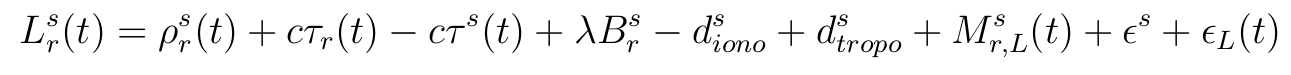
\includegraphics[scale=0.3]{ec17.png}
		    \caption{Rango de Portadora}
		    \label{fig:EcRangoPortadora}
	\end{figure}


Puede apreciarse que el modelo de la Ec X, es similar al modelo observacional planteado para el pseudorango. Sin embargo, se diferencia por el signo opuesto al considerar el término del retraso ionosférico y la adición de un término para la compensación del rango de la señal satelital \begin{shaded}$\Lambda$ ** OJO Lamdda**. El signo opuesto que acompaña al retraso ionosférico está asociado con el fenómeno de divergencia ionosférica que influye sobre el observable en cuestión.
\end{shaded}

\subsection{Posicionamiento Absoluto (Absolute Positioning)}

En realidad, los modelos de portadora por sí solos raramente son empleados para el cálculo de posición de un receptor GPS. En cambio modelos como el caso del posicionamiento absoluto se apoyan en la idea de tomar puntos de referencia en el espacio (ubicación de los satélites) y las distancias hasta el punto en el cual se desea conocer la posición (receptor). 

	\begin{figure}[ht]
		    \centering
		    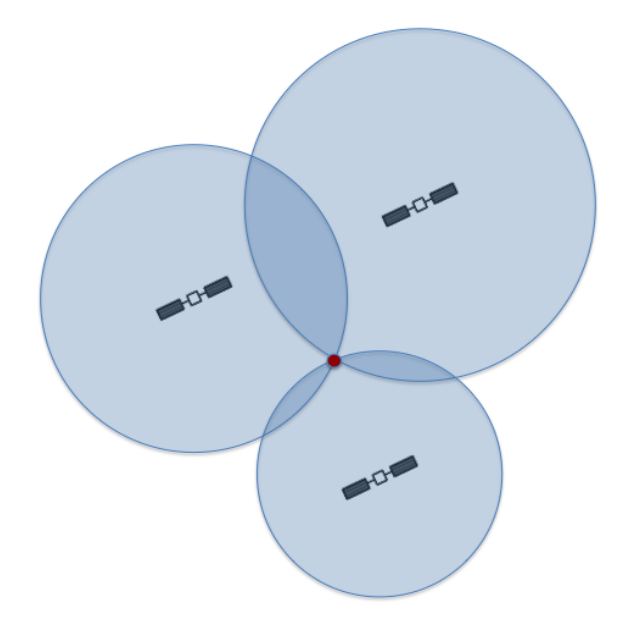
\includegraphics[scale=0.3]{Trilateracion.png}
		    \caption{El concepto de Trilateración}
		    \label{fig:Trilateracion}
	\end{figure}

La \textbf{fig tal} da una idea más clara del concepto de trilateración \textbf{[ref 23]}, donde el objeto es encontrar el punto de intersección de un conjunto de esferas con un centro de coordenadas conocido (posición del satélite) y el rango de alcance en señal de los satélites (radio).  Es importante aclarar es que la determinación del punto de intersección entre el rango de alcance de los satélites es válido para un cierto instante de tiempo, ya que el receptor tiene libertad de moverse a lo largo del espacio. \\

Por otra parte, el cálculo o determinación del punto de intersección entre las esferas para un determinado instante de tiempo tiene un nivel de incertidumbre debido a los errores que influyen en los observables, como son por ejemplo la orientación geométrica del satélite y el error en el reloj del receptor, producto de esta incertidumbre es probable que las esferas en algunos casos no se intersecten o se intersecten en varios puntos donde posiblemente esté ubicado el receptor.\\

El espacio tridimensional en donde puede ser posible ubicar el receptor está asociado con el término dilución de la precisión (GDOP, VDOP, etc).\\

	\begin{figure}[ht]
		    \centering
		    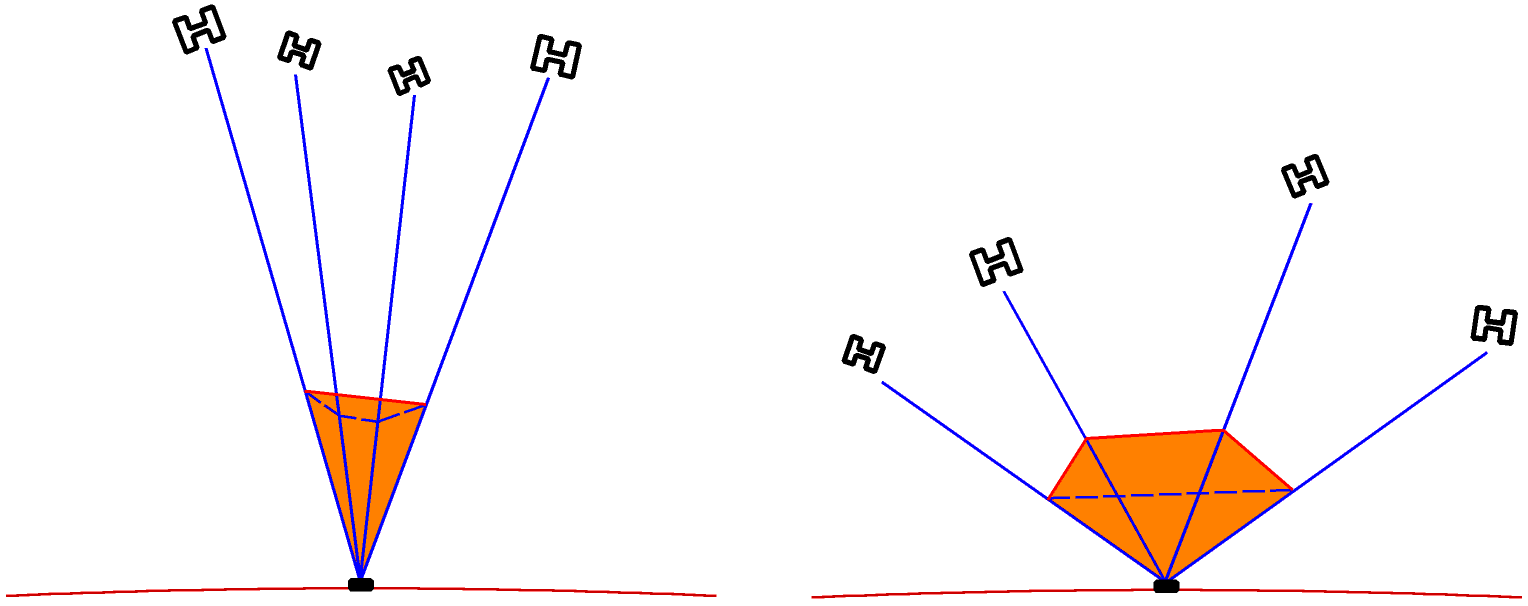
\includegraphics[scale=0.2]{GDOP.png}
		    \caption{Concepto de GDOP.}
		    \label{fig:DOP}
	\end{figure}


El error de sincronización de reloj puede desencadenar errores del orden de 300 km en posicionamiento, razón por la cual es considerado como un parámetro de posicionamiento que impone la restricción de mínimo 4 satélites a la vista para llevar a cabo tareas de posicionamiento con niveles de incertidumbre bajos.

Asumiendo que se corrigen todos los errores que influyen sobre el pseudo-rango a excepción del término de compensación de reloj local, la ecuación que expresara el pseudo-rango es:

%Ec18 pág 32
	\begin{figure}[ht]
		    \centering
		    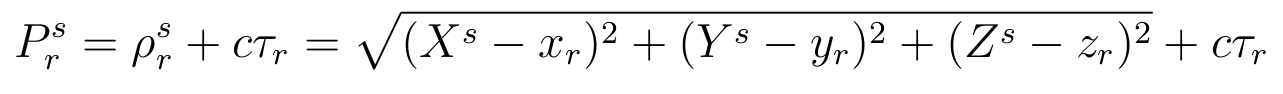
\includegraphics[scale=0.3]{ec18.png}
		    \caption{Pseudorango + incertidumbre}
		    \label{fig:EcPseudoIncert}
	\end{figure}

	\begin{figure}[ht]
		    \centering
		    \normalcolor
		    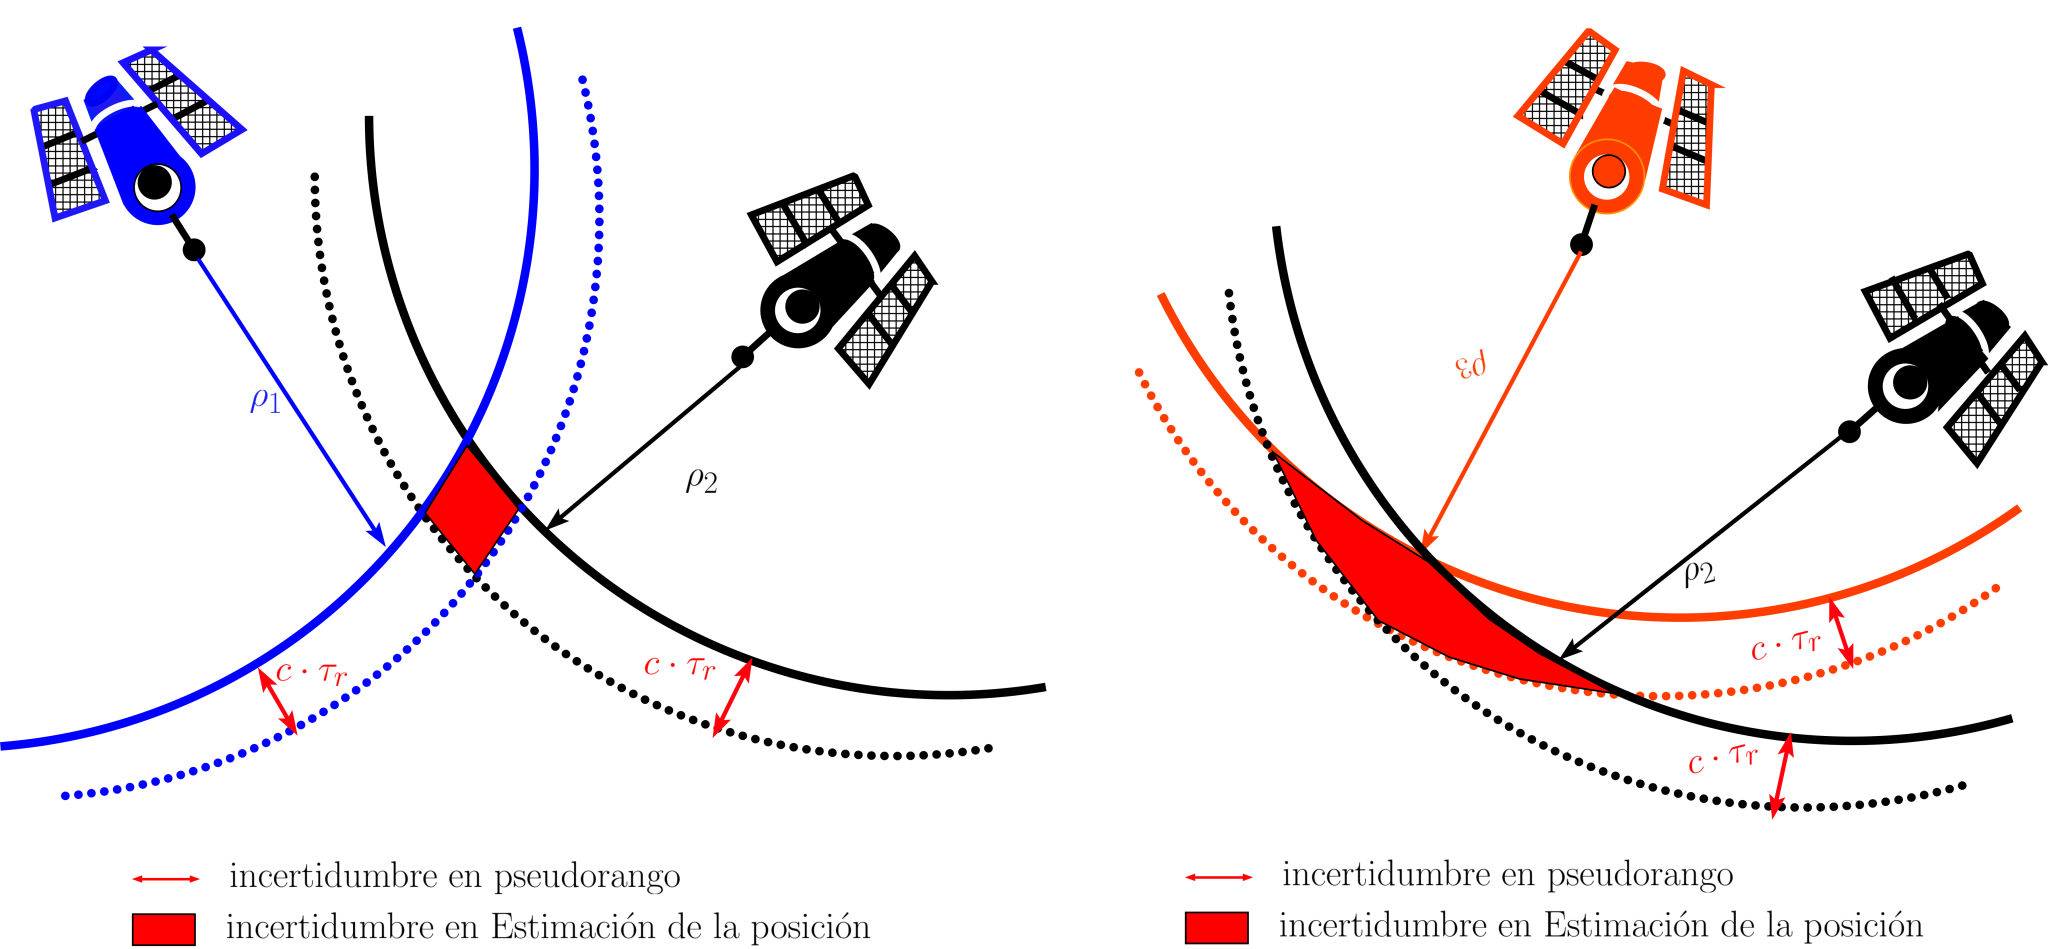
\includegraphics[scale=0.18]{IncertidumbreVsDOP.png}
		    \caption{Incertidumbre en posicionamiento, error en reloj.}
		    \label{fig:IncertidumbrePosicionGPS}
	\end{figure}
	
De la expresión anterior se pueden identificar claramente 4 incógnitas, que pueden ser resueltas a partir de las observaciones obtenidas desde n satélites (Pr1, Pr2, ... Prn). Donde la disponibilidad de satélites es superior al requerimiento de 4 satélites para dar solución al problema de 4 incógnitas. Producto de ello, el sistema de ecuaciones conformado por n satélites y 4 incógnitas es conocido como problema sobre determinado (overdetermined) y suele ser resuelto por medio de la minimización del término \textit{$e = c*t$} por medio de minimización de mínimos cuadrados (Least-squares).


\subsection{Los tipos de receptores GPS}

En un principio  los dispositivos empleados para llevar a cabo tareas de posicionamiento eran dispositivos electrónicos complejos encargados de recibir y procesar las señales de radiofrecuencia enviadas por los satélites para determinar la posición del receptor sobre la tierra.\\

Con la aparición de nuevos procesos Impresión y manufactura de dispositivos electrónicos, se dio auge a los sistemas embebidos, pequeños dispositivos de cómputo  con capacidad para interactuar con módulos y dispositivos de hardware y ejecutar tareas de software, con esta capacidad de interacción dual Software-Hardware.\\

El escenario en el cual las tareas de software reemplazan funcionalidades de Hardware es conocido como radio definido por software SDR. El uso de paquetes de software SDR permite centrar la atención en perfeccionar el diseño de los dispositivos encargados de la adquisición de señales de radiofrecuencia para contar con señales de mayor fidelidad.\\

Adicionalmente SDR brinda mayor flexibilidad para el desarrollo de nuevas formas de procesamiento de señales basadas en DSP, reduciendo así la complejidad y costo de los dispositivos de comunicaciones. En el caso particular de los sistemas de navegación satelital, el uso de SDR se ha convertido en una herramienta que facilita el prototipado de receptores GPS de manera independiente al hardware.\\

Básicamente los receptores de GPS se pueden clasificar en tres familias.

\begin{itemize}

\item Receptores de electrónica de consumo: Dispositivos económicos que influyen pantalla para el despliegue de resultados y una antena microondas para la recepción de señal,.Básicamente son dispositivos con la funcionalidad de Hardware para la adquisición de Señales satelitales y uno o varios dispositivos de entrada para la  interacción con el usuario (Ej. Celulares)

\item Receptores basados en electrónica embebida: son equipos diseñados y manufacturados específicamente para aplicaciones de posicionamiento, que cuentan con la funcionalidad de Hardware para la adquisición de Señales satelitales y que por lo general no cuentan con interfaz de interacción con el usuario.

\item Receptores basados en software: No es claramente y conocidos Como “radio definido por software SDR”, que buscan minimizar el hardware requerido para la adquisición y procesamiento de señales satelitales, apoyados en técnicas de procesamiento de Señales implementadas en rutinas de software.

\end{itemize}
